\documentclass[11pt]{amsart}
\usepackage{amsmath,amssymb,amsthm}
\usepackage[margin=1.1in]{geometry}
\usepackage{hyperref}
\usepackage{booktabs}
\usepackage{graphicx}
\graphicspath{{../figures/}{figures/}}

\newtheorem{theorem}{Theorem}[section]
\newtheorem{proposition}[theorem]{Proposition}
\newtheorem{lemma}[theorem]{Lemma}
\newtheorem{corollary}[theorem]{Corollary}
\theoremstyle{remark}
\newtheorem{remark}[theorem]{Remark}

\newcommand{\cA}{\mathcal{A}}
\newcommand{\cB}{\mathcal{B}}
\newcommand{\cE}{\mathcal{E}}
\newcommand{\cP}{\mathcal{P}}
\newcommand{\cT}{\mathcal{T}}
\newcommand{\Sg}{\mathfrak{S}}
\newcommand{\li}{\operatorname{li}}
\newcommand{\verify}[1]{\textbf{[verify: #1]}}

\title[Almost prime sums of two squares]{On primes $p$ for which $N-p$ is an almost prime sum of two squares}
\author{Ruqing Chen}
\address{GUT Geoservice Inc., Montreal, Canada}
\email{ruqing@hotmail.com}
\date{\today}

\begin{document}

\begin{abstract}
Let $N$ be a sufficiently large even integer. We show that the number of primes $p\le N$ such that
$N-p$ is a sum of two squares having at most nine prime factors, counted with multiplicity, is
$\gg \Sg(N)N/(\log N)^2$. The proof follows the vector sieve framework of Nath and Xie, combining two
semi-linear sieves at the Bombieri--Vinogradov level of distribution with Richert's logarithmic weights.
Integers with two large prime factors $\equiv 3 \pmod 4$, which escape the semi-linear sieve, are removed by
a switching argument. The final numerical inequality is verified with outward-rounded interval arithmetic.
\end{abstract}

\maketitle

%=====================================================================================================
\section{Introduction}

Chen's theorem \cite{Chen} states that every sufficiently large even integer $N$ is of the form
$N=p+P_2$, where $P_2$ has at most two prime factors. Linnik \cite{Linnik} showed that every sufficiently
large integer is of the form $p+x^2+y^2$, and Iwaniec \cite{IwaniecQF} and Motohashi \cite{Motohashi70}
studied primes $p$ with $p-1$ a sum of two squares by sieve methods; the semi-linear (half-dimensional)
sieve of Iwaniec \cite{IwaniecHalf} is the natural tool for the condition ``$n$ is a sum of two squares''.
More recently Nath and Xie \cite{NathXie} combined a semi-linear and a linear sieve in a vector sieve
\cite{BF} to show that there are $\gg x/(\log x)^{5/2}$ primes $p\le x$ such that $p-1$ is a sum of two
squares and $\Omega(p+2)\le 11$.

In this note we consider the additive problem in which both conditions are imposed on the \emph{same}
shifted number $N-p$.

\begin{theorem}\label{thm:main}
There is an absolute constant $N_0$ such that for every even $N\ge N_0$,
\[
\#\{p\le N:\ N-p=x^2+y^2 \text{ for some } x,y\in\mathbb Z,\ \Omega(N-p)\le 9\}
\ \ge\ \frac{1}{10}\,\Sg(N)\,\frac{N}{(\log N)^2},
\]
where $\Sg(N)=2\prod_{\ell>2}\bigl(1-(\ell-1)^{-2}\bigr)\prod_{\ell\mid N,\ \ell>2}\frac{\ell-1}{\ell-2}$
is the binary Goldbach singular series. The constant $N_0$ is ineffective.
\end{theorem}

\subsection*{Method}
Write $n=N-p$ and restrict to $p\equiv N-1\pmod 4$, so that $n\equiv 1\pmod 4$. If $n$ has no prime
factor $q\equiv 3\pmod 4$ at all, then $n$ is a sum of two squares. With the Bombieri--Vinogradov level
$N^{1/2}$ one cannot sift the primes $q\equiv3\pmod 4$ all the way up to $N^{1/2}$: the semi-linear
lower bound function satisfies $f_{1/2}(s)=0$ for $s\le 1$. We therefore sift them only up to
$y=N^{1/2-\delta}$. Since $n\equiv 1\pmod 4$, a survivor then has either no prime factor $\equiv 3\pmod 4$,
or exactly two, both $\ge y$; the latter are counted from above by switching the roles of $p$ and
$q_1q_2m$ (Section~\ref{sec:switch}). The number of prime factors is controlled by Richert's logarithmic
weights (Section~\ref{sec:weights}). The resulting numerical inequality is verified rigorously in
Section~\ref{sec:numerics}.

\begin{remark}
We have not found the statement of Theorem~\ref{thm:main} in the literature, but our search was limited
\verify{MathSciNet/zbMATH search and correspondence with experts}. The method is a direct adaptation of
\cite{NathXie}; the only additional ingredient is the switching step of Section~\ref{sec:switch}.
\verify{check how \cite{NathXie} treat the $s=1$ barrier of the semi-linear sieve}.
\end{remark}

%=====================================================================================================
\section{Notation and tools}

Throughout, $N$ is a large even integer, $\varepsilon>0$ is small, $p,q,\ell$ denote primes,
$\cP_1=\{q\equiv 1 \pmod 4\}$, $\cP_3=\{q\equiv 3\pmod 4\}$, and for a set of primes $\cP$ we write
$P(\cP;z)=\prod_{q\in\cP,\,q<z}q$. Let
\[
\cA=\{\,n=N-p:\ p\le N,\ p\equiv N-1 \ (\mathrm{mod}\ 4)\,\},\qquad X=\tfrac12\li(N).
\]
For odd squarefree $d$ put $g(d)=\prod_{\ell\mid d}g(\ell)$ with $g(\ell)=1/(\ell-1)$ if $\ell\nmid N$ and
$g(\ell)=0$ if $\ell\mid N$, and define $r_d$ by $\#\{n\in\cA: d\mid n\}=Xg(d)+r_d$.

\begin{lemma}[Bombieri--Vinogradov with divisor weights]\label{lem:BV}
For every $A>0$ there is $B=B(A)$ such that, with $D=N^{1/2}(\log N)^{-B}$,
\[
\sum_{d\le D}\mu^2(d)\,\tau_3(d)\,|r_d|\ \ll_A\ \frac{N}{(\log N)^A}.
\]
\end{lemma}

\begin{proof}
For odd $d$ with $(d,N)=1$, $\#\{n\in\cA:d\mid n\}=\pi(N;4d,a_d)$ for a residue $a_d$ coprime to $4d$, and
$\varphi(4d)=2\varphi(d)$; for $(d,N)>1$ the count is $O(1)$. Hence $|r_d|\le E(N;4d)+O(1)$ with
$E(N;k)=\max_{(a,k)=1}|\pi(N;k,a)-\li(N)/\varphi(k)|$. By Brun--Titchmarsh,
$|r_d|\ll N/(\varphi(d)\log N)$ for $d\le D$. By Cauchy--Schwarz,
\[
\sum_{d\le D}\tau_3(d)|r_d|\le\Bigl(\sum_{d\le D}\tau_3(d)^2|r_d|\Bigr)^{1/2}\Bigl(\sum_{d\le D}|r_d|\Bigr)^{1/2}
\ll \Bigl(N(\log N)^{C}\Bigr)^{1/2}\Bigl(\frac{N}{(\log N)^{2A+C}}\Bigr)^{1/2},
\]
using $\sum_{d\le D}\tau_3(d)^2/\varphi(d)\ll(\log N)^{C}$ and the Bombieri--Vinogradov theorem
\cite{Bombieri} for the moduli $4d\le 4D$.
\end{proof}

\begin{lemma}[The semi-linear sieve]\label{lem:semi}
Let $F=F_{1/2}$, $f=f_{1/2}$ be the continuous solutions of
\[
(\sqrt s\,F(s))'=\tfrac{1}{2\sqrt s}\,f(s-1),\qquad (\sqrt s\,f(s))'=\tfrac{1}{2\sqrt s}\,F(s-1)\qquad(s>1),
\]
with $F(s)=A/\sqrt s$ for $0<s\le 2$, $f(s)=0$ for $s\le 1$, and $A=2\sqrt{e^{\gamma}/\pi}$. Then
$f(s)=A\,\mathrm{arccosh}(\sqrt s)/\sqrt s$ for $1\le s\le 3$, $F$ is decreasing, $f$ is increasing, and
$F(s),f(s)\to 1$. Let $\cP\in\{\cP_1,\cP_3\}$. For $z\le D$ and $s=\log D/\log z$ there are
upper and lower sieve weights $\lambda_d^{\pm}$, $|\lambda^\pm_d|\le 1$, supported on
$d\mid P(\cP;z)$, $d\le D$, with $\sum_{d\mid (n,P(\cP;z))}\lambda^-_d\le 1_{(n,P(\cP;z))=1}\le
\sum_{d\mid (n,P(\cP;z))}\lambda^+_d$ and
\[
\sum_d\lambda^{\pm}_d g(d)=V(\cP;z)\bigl(F(s)\ \text{resp.}\ f(s)+o(1)\bigr),\qquad
V(\cP;z)=\prod_{q\in\cP,\ q<z}(1-g(q)).
\]
\end{lemma}

\begin{proof}
This is Iwaniec's $\beta$-sieve with $\kappa=1/2$, $\beta=1$ \cite{IwaniecHalf,IwaniecRosser};
see also \cite[Ch.~11, 14]{OC}. The sets $\cP_1,\cP_3$ have sifting density $1/2$ by the prime number
theorem in progressions modulo $4$. The closed form on $[1,3]$ follows by integrating the second equation.
\verify{asymptotic equality of the main terms in the form used in \cite[Prop.~3.10]{NathXie}}
\end{proof}

Figure~\ref{fig:semilinear} shows $F_{1/2}$ and $f_{1/2}$. Since $f_{1/2}(s)=0$ for $s\le 1$, sifting the
primes $q\equiv 3\pmod 4$ up to $N^{1/2}$ with level $N^{1/2}$ gives no lower bound; this is why we sift
them only up to $N^{1/2-\delta}$ in Section~\ref{sec:weights}.

\begin{figure}[htbp]
\centering
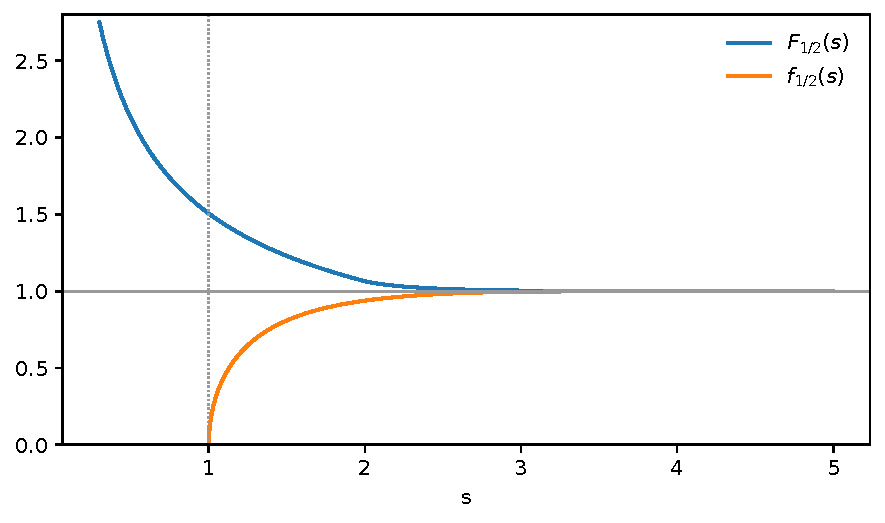
\includegraphics[width=0.82\textwidth]{semilinear_sieve_functions.pdf}
\caption{The semi-linear sieve functions $F_{1/2}(s)$ and $f_{1/2}(s)$ (dimension $\kappa=1/2$, sieving
limit $\beta=1$). The lower bound function vanishes for $s\le 1$, so at the Bombieri--Vinogradov level
$\theta=1/2$ the primes $q\equiv 3\pmod 4$ cannot be sifted all the way up to $N^{1/2}$.}
\label{fig:semilinear}
\end{figure}

\begin{lemma}[Vector sieve]\label{lem:vector}
Let $a,b\in\{0,1\}$ and $a^-\le a\le a^+$, $b^-\le b\le b^+$ with $a^+,b^+\ge 0$. Then
$ab\ge a^-b^++a^+b^--a^+b^+$ and $ab\le a^+b^+$.
\end{lemma}

\begin{proof}
$(a^+-a)(b^+-b)\ge 0$ gives $ab\ge a^+b+ab^+-a^+b^+$, and $a^+b\ge a^+b^-$, $ab^+\ge a^-b^+$.
\end{proof}

\begin{lemma}[Bombieri--Vinogradov for convolutions]\label{lem:conv}
Let $\alpha_k,\beta_l$ be complex coefficients bounded by divisor functions, supported on
$K<k\le 2K$ and $l\le N/K$ with $N^{\varepsilon}\le K\le N^{1-\varepsilon}$, and suppose $\beta$ satisfies
the Siegel--Walfisz condition. Then for every $A>0$ there is $B$ with
\[
\sum_{d\le N^{1/2}(\log N)^{-B}}\ \max_{(a,d)=1}\Bigl|\sum_{\substack{kl\le N\\ kl\equiv a\ (d)}}\alpha_k\beta_l
-\frac{1}{\varphi(d)}\sum_{\substack{kl\le N\\ (kl,d)=1}}\alpha_k\beta_l\Bigr|\ll\frac{N}{(\log N)^A}.
\]
\end{lemma}

\begin{proof}
The result follows from the bilinear mean value theorem of Pan--Ding--Wang \cite[Lemma~2]{PDW} and
Motohashi \cite[Theorem~1]{Motohashi76} for general convolutions with moduli up to
$N^{1/2}(\log N)^{-B}$; see also \cite[Theorem~0]{BFI} for an explicit statement.
\end{proof}

%=====================================================================================================
\section{The weighted vector sieve}\label{sec:weights}

Fix parameters $0<\alpha<2\delta<1/2$, $\delta<1/4$, $0<\lambda$, $\alpha<\beta_1\le 1/2$, and put
\[
y=N^{1/2-\delta},\qquad z_0=N^{\alpha},\qquad y_1=N^{\beta_1},\qquad P=P(\cP_3;y)\,P(\cP_1;z_0).
\]
Note that every odd prime $q<z_0$ divides $P$. For $n\in\cA$ with $(n,P)=1$ define
\[
w_n=1-\lambda\sum_{\substack{q\mid n,\ q\in\cP_1\\ z_0\le q<y_1}}\Bigl(1-\frac{\log q}{\log y_1}\Bigr),
\qquad W=\sum_{\substack{n\in\cA\\ (n,P)=1}}w_n .
\]

\begin{lemma}[Structure of the survivors]\label{lem:structure}
Let $n\in\cA$ with $(n,P)=1$. Then exactly one of the following holds:
\begin{enumerate}
\item[(i)] all prime factors of $n$ lie in $\cP_1$, or $n=q^2m$ with $q\in\cP_3$; in both cases $n$ is a
sum of two squares;
\item[(ii)] $n=q_1q_2m$ with $q_1<q_2$, $q_1,q_2\in\cP_3$, $q_1\ge y$, and $m\le N^{2\delta}$ composed of
primes of $\cP_1$ that are $\ge z_0$.
\end{enumerate}
\end{lemma}

\begin{proof}
$n$ is odd and $n\equiv1\pmod 4$, so the number of prime factors of $n$ in $\cP_3$, counted with
multiplicity, is even. All of them are $\ge y$, and $y^4>N$ because $\delta<1/4$; so there are $0$ or $2$
of them. If there are none, or the two coincide, $n$ is a sum of two squares by Fermat's theorem. Otherwise
we are in case (ii), and $m=n/(q_1q_2)\le N/y^2=N^{2\delta}$; its prime factors are in $\cP_1$ and
$\ge z_0$ because $(n,P)=1$.
\end{proof}

\begin{lemma}[Counting prime factors]\label{lem:omega}
Let $n$ be as in Lemma~\ref{lem:structure}(i), squarefree, and suppose $w_n>0$. Then
$\Omega(n)<1/\lambda+1/\beta_1$.
\end{lemma}

\begin{proof}
All prime factors of $n$ are in $\cP_1$ and are $\ge z_0$. Terms with $q\ge y_1$ satisfy
$1-\log q/\log y_1\le 0$, hence
\[
\sum_{\substack{q\mid n\\ z_0\le q<y_1}}\Bigl(1-\frac{\log q}{\log y_1}\Bigr)\ \ge\
\sum_{q\mid n}\Bigl(1-\frac{\log q}{\log y_1}\Bigr)=\Omega(n)-\frac{\log n}{\log y_1}\ \ge\
\Omega(n)-\frac{1}{\beta_1}.
\]
Thus $w_n>0$ forces $\lambda(\Omega(n)-1/\beta_1)<1$.
\end{proof}

The elements $n\in\cA$ divisible by $q^2$ for some prime $q\ge z_0$ number at most
$\sum_{z_0\le q\le\sqrt N}(N/q^2+1)\ll N^{1-\alpha}$, which is negligible.

\begin{proposition}\label{prop:W}
Let $\theta_3\in(0,1/2)$ and, for each $u\in[\alpha,\beta_1]$, let $t(u)\in(0,1/2-u)$. Put
$s_3=\theta_3/(1/2-\delta)$, $s_1=(1/2-\theta_3)/\alpha$,
\[
L=f(s_3)F(s_1)+F(s_3)f(s_1)-F(s_3)F(s_1),
\]
\[
R=\frac12\int_{\alpha}^{\beta_1}\Bigl(1-\frac{u}{\beta_1}\Bigr)
F\Bigl(\frac{t(u)}{1/2-\delta}\Bigr)F\Bigl(\frac{1/2-u-t(u)}{\alpha}\Bigr)\frac{du}{u}.
\]
Then
\[
W\ \ge\ \bigl(L-\lambda R+o(1)\bigr)\,\frac{1}{2e^{\gamma}\sqrt{\alpha(1/2-\delta)}}\;\Sg(N)\frac{N}{(\log N)^2}.
\]
\end{proposition}

\begin{proof}
Write $a=1_{(n,P(\cP_3;y))=1}$, $b=1_{(n,P(\cP_1;z_0))=1}$, and let $a^\pm$, $b^\pm$ be the sums of the
semi-linear sieve weights of Lemma~\ref{lem:semi} of levels $D_3=N^{\theta_3}$ and
$D_1=N^{1/2-\theta_3}(\log N)^{-B}$. By Lemma~\ref{lem:vector},
\[
\sum_{\substack{n\in\cA\\(n,P)=1}}1\ \ge\ \sum_{n\in\cA}(a^-b^++a^+b^--a^+b^+).
\]
Since the prime sets are disjoint, $g(de)=g(d)g(e)$ for $d\mid P(\cP_3;y)$, $e\mid P(\cP_1;z_0)$, and
\[
\sum_{n\in\cA}a^-b^+=X\Bigl(\sum_d\lambda^-_dg(d)\Bigr)\Bigl(\sum_e\lambda^+_eg(e)\Bigr)
+O\Bigl(\sum_{m\le D}\tau(m)|r_m|\Bigr),
\]
and similarly for the other two terms. By Lemma~\ref{lem:semi} the main terms combine to
\[
XV(\cP_3;y)V(\cP_1;z_0)\bigl(L+o(1)\bigr),
\]
and by Lemma~\ref{lem:BV} the error is $O(N(\log N)^{-A})$.

For the weights, fix $q\in\cP_1$, $q=N^u$ with $\alpha\le u<\beta_1$. By Lemma~\ref{lem:vector}, the
number of $n\in\cA$ with $q\mid n$ and $(n,P)=1$ is at most $\sum_{n\in\cA,\,q\mid n}a^+_qb^+_q$, where
$a_q^+$, $b_q^+$ are upper weights of levels $N^{t(u)}$ and $N^{1/2-u-t(u)}(\log N)^{-B}$. This is
\[
Xg(q)V(\cP_3;y)V(\cP_1;z_0)\Bigl(F\Bigl(\tfrac{t(u)}{1/2-\delta}\Bigr)F\Bigl(\tfrac{1/2-u-t(u)}{\alpha}\Bigr)
+o(1)\Bigr)+O\Bigl(\sum_{m\le D/q}\tau(m)|r_{qm}|\Bigr).
\]
Summing over $q$, the error terms total $\ll\sum_{m\le D}\tau_3(m)|r_m|\ll N(\log N)^{-A}$ by
Lemma~\ref{lem:BV}, and the prime number theorem modulo $4$ turns
$\sum_{q\in\cP_1}g(q)(1-\log q/\log y_1)(\cdots)$ into $R+o(1)$ (the class $\cP_1$ has density $1/2$).
Since the integrand involves $F(s)\le A/\sqrt s$ only as $s\to 0^+$, the integral converges.

Finally, by Mertens' theorem and its analogue in progressions modulo 4,
\[
V(\cP_3;y)V(\cP_1;z_0)=\prod_{\substack{2<q<z_0}}(1-g(q))\prod_{\substack{q\in\cP_3\\ z_0\le q<y}}(1-g(q))
\sim\frac{\Sg(N)e^{-\gamma}}{\alpha\log N}\Bigl(\frac{\alpha}{1/2-\delta}\Bigr)^{1/2},
\]
and $X\sim N/(2\log N)$, which gives the stated normalisation.
\end{proof}

%=====================================================================================================
\section{Switching}\label{sec:switch}

Let $\cE$ be the set of $p\le N$, $p\equiv N-1\pmod 4$, such that $n=N-p$ satisfies $(n,P)=1$ and falls
under Lemma~\ref{lem:structure}(ii). Let $\cT$ be the set of triples $(q_1,q_2,m)$ with $q_1<q_2$,
$q_i\in\cP_3$, $q_1\ge y$, $q_1q_2m\le N$, and $m$ composed of primes of $\cP_1$ that are $\ge z_0$
(so $m\le N^{2\delta}$), and let $\cB$ be the multiset $\{N-q_1q_2m:(q_1,q_2,m)\in\cT\}$.

\begin{proposition}\label{prop:switch}
We have $\#\cE\le\bigl(4c(\delta,\alpha)+o(1)\bigr)\Sg(N)N/(\log N)^2$, where
\[
c(\delta,\alpha)=\frac14\int_{[0,2\delta]}\ \frac{1}{1-\mu}\log\frac{1/2+\delta-\mu}{1/2-\delta}\ d\nu(\mu),
\qquad
\nu=\sum_{j\ge0}\frac{\nu_1^{*j}}{j!},\quad d\nu_1(\mu)=\tfrac12\,1_{[\alpha,2\delta]}(\mu)\frac{d\mu}{\mu},
\]
($\nu_1^{*0}$ is the unit mass at $0$, and $\nu$ is restricted to $[0,2\delta]$).
\end{proposition}

\begin{proof}
Every $p\in\cE$ is a prime element of $\cB$, and an element $b\in\cB$ with $b\ge D=N^{1/2}(\log N)^{-B}$
that is prime is coprime to $P(D)=\prod_{2<\ell<D}\ell$ (all elements of $\cB$ are odd). Hence
\[
\#\cE\le S(\cB,D)+\#\{t\in\cT:N-t<D\},\qquad S(\cB,D)=\#\{b\in\cB:(b,P(D))=1\}.
\]
The last term is $\ll D\,N^{\varepsilon}$. For odd squarefree $d$ write
$\#\{b\in\cB:d\mid b\}=|\cB|g_\cB(d)+r_\cB(d)$ with $g_\cB(\ell)=1/(\ell-1)$ for $\ell\nmid N$, $g_\cB(\ell)=0$
for $\ell\mid N$, $\ell<z_0$. (Primes $\ell\mid N$ with $\ell\ge z_0$ are at most $1/\alpha$ in number and
change the main term by a factor $1+o(1)$.) The sequence $t=q_1\cdot(q_2m)$ is a convolution with $q_1$
in $[N^{1/2-\delta},N^{1/2}]$. We split the ranges of $q_1$, $q_2$ and $m$ dyadically into
$O((\log N)^3)$ boxes. In each box the conditions $q_1<q_2$ and $q_1q_2m\le N$ are removed by Perron's
formula (or a smooth partition of unity), at the cost of a factor $(\log N)^{C}$ and an admissible error
term; the resulting sequences are convolutions to which Lemma~\ref{lem:conv} applies, with
$q_1$ carrying the Siegel--Walfisz condition. Taking $A$ large in Lemma~\ref{lem:conv} we obtain
$\sum_{d\le D}|r_\cB(d)|\ll N(\log N)^{-A}$.
The upper bound linear sieve at level $D$ with sifting range $z=D$, i.e.\ $s=1$, gives
\[
S(\cB,D)\le|\cB|\,V_\cB(D)\,(F_1(1)+o(1))+O\Bigl(\sum_{d\le D}|r_\cB(d)|\Bigr),\qquad F_1(1)=2e^{\gamma}.
\]
Here
\[
V_\cB(D)=\prod_{2<\ell<D}\bigl(1-g_\cB(\ell)\bigr)\sim\frac{\Sg(N)e^{-\gamma}}{\log D},
\]
and $\log D\sim\frac12\log N$, so $S(\cB,D)\le(4+o(1))\Sg(N)|\cB|/\log N$.

It remains to evaluate $|\cB|=|\cT|$. Writing $m=N^{\mu}$, $q_1=N^{u}$ and using the prime number
theorem in progressions modulo 4 for $q_1$ and $q_2$,
\[
|\cT|=\sum_m\ \sum_{\substack{q_1\in\cP_3\\ y\le q_1<\sqrt{N/m}}}\pi\Bigl(\frac{N}{mq_1};4,3\Bigr)(1+o(1))
=\frac{N}{\log N}\Bigl(\sum_m\frac1m\cdot\frac14\int_{1/2-\delta}^{(1-\mu)/2}\frac{du}{u(1-\mu-u)}+o(1)\Bigr),
\]
and $\int_{1/2-\delta}^{(1-\mu)/2}\frac{du}{u(1-\mu-u)}=\frac{1}{1-\mu}\log\frac{1/2+\delta-\mu}{1/2-\delta}$.
The sum over $m$ (products of $j$ primes of $\cP_1$ in $[z_0,N^{2\delta}]$, $j\ge0$) is bounded above by
the integral against $\nu$ (dropping the distinctness of the prime factors only increases it), by
Mertens' theorem modulo 4. This gives $|\cB|\le(c(\delta,\alpha)+o(1))N/\log N$.
\end{proof}

%=====================================================================================================
\section{Numerical verification and proof of Theorem~\ref{thm:main}}\label{sec:numerics}

By Lemma~\ref{lem:structure}, the survivors split into the set of case (i), on which $w_n$ is the weight
we want, and the set of case (ii), which corresponds to $\cE$. Since $w_n\le 1$,
\[
\sum_{\substack{n\in\cA,\ (n,P)=1\\ \text{case (i)}}}w_n\ \ge\ W-\#\cE .
\]
By Propositions~\ref{prop:W} and~\ref{prop:switch} the right-hand side is at least
$(\mathrm{net}+o(1))\Sg(N)N/(\log N)^2$, where
\[
\mathrm{net}=\frac{L-\lambda R}{2e^{\gamma}\sqrt{\alpha(1/2-\delta)}}-4c(\delta,\alpha).
\]
We choose
\[
\delta=\tfrac{1}{10},\quad \alpha=\tfrac{7}{1000},\quad \lambda=\tfrac{3}{20},\quad \beta_1=\tfrac{3}{10},
\quad \theta_3=0.478,
\]
so that $1/\lambda+1/\beta_1=20/3+10/3=10$ and, by Lemma~\ref{lem:omega}, every squarefree case-(i)
survivor with $w_n>0$ has $\Omega(n)\le 9$.

\begin{lemma}\label{lem:numerics}
For these parameters, $L\ge 0.583795$, $R\le 2.050122$, $c(\delta,\alpha)\le 0.339858$ and
$\mathrm{net}\ge 0.106297$.
\end{lemma}

\begin{proof}[Method of verification]
The computation is carried out by the accompanying script \texttt{certify.py}.
\begin{enumerate}
\item On $(0,2]$ and $[1,3]$, $F$ and $f$ are evaluated from their closed forms in interval arithmetic
(\texttt{mpmath.iv}, 80 bits). For $s\in[2,80]$ the two delay equations are integrated on the grid
$s\in 10^{-3}\mathbb Z$: on each step the lagged function is enclosed between its values at the two
end points (by monotonicity), and $\int ds/(2\sqrt s)$ is computed exactly. Each floating point operation
is followed by one outward rounding step, which is sufficient since $+,-,\times,/,\sqrt{\ }$ are correctly
rounded in IEEE~754. For non-grid arguments, monotonicity gives one-sided bounds from neighbouring grid
points.
\item $L$ is bounded below using $L=f(s_3)F(s_1)+F(s_3)(f(s_1)-F(s_1))$ and $f(s_1)-F(s_1)\le 0$.
\item $R$ is bounded above by a Riemann sum over $6000$ cells, with $t(u)$ constant on each cell; on a cell
$[u_a,u_b]$ the factor $(1-u/\beta_1)/u$ is largest at $u_a$ and $F((1/2-u-t)/\alpha)$ is largest at $u_b$.
\item For $c$, the measure $\nu_1$ is replaced by masses $\frac12\log\frac{k+1}{k}$ placed at the left end
points $k/2000$ of the cells; the convolution powers then dominate $\nu$ on initial segments. The
integrand $I(\mu)=\frac{1}{1-\mu}\log\frac{0.6-\mu}{0.4}$ is decreasing on $[0,0.2]$ (its derivative has the
sign of $I(\mu)-1/(0.6-\mu)<0$), so moving mass to the left gives an upper bound. The floating point
convolution is multiplied by $1+10^{-9}$.
\end{enumerate}
\end{proof}

\begin{proof}[Proof of Theorem~\ref{thm:main}]
By Lemma~\ref{lem:numerics} and the discussion above, for $N$ large,
$\sum_{\text{case (i)}}w_n\ge 0.106\,\Sg(N)N/(\log N)^2$. Removing the $\ll N^{1-\alpha}$ non-squarefree
elements, each remaining $n$ with $w_n>0$ is a sum of two squares with $\Omega(n)\le 9$, and since
$w_n\le1$ the number of such $n$, i.e.\ of primes $p$, is at least $\frac1{10}\Sg(N)N/(\log N)^2$.
The constant $N_0$ is ineffective because of the Siegel--Walfisz theorem underlying Lemmas~\ref{lem:BV}
and~\ref{lem:conv}.
\end{proof}

\begin{remark}
Floating point computations (not certified) indicate that without Richert's weights ($\lambda=0$) the
same method gives $\Omega(n)\le 24$, and that with the switching constant $5$ in place of $4$ it still gives
$\Omega(n)\le 11$; see Figure~\ref{fig:comparison}.
\end{remark}

\begin{figure}[htbp]
\centering
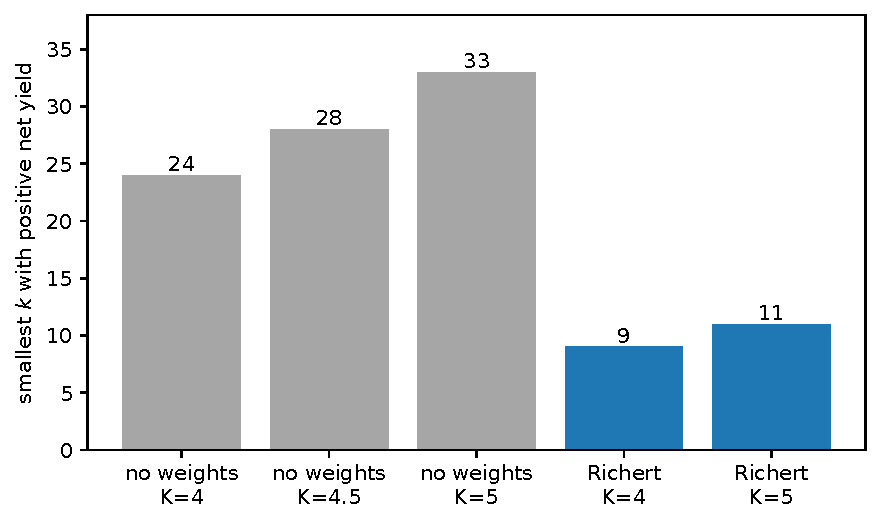
\includegraphics[width=0.82\textwidth]{smallest_k_by_scheme.pdf}
\caption{Smallest bound $k$ for $\Omega(N-p)$ obtained by floating-point parameter scans, without weights
and with Richert's weights, for several values of the switching constant $K$. Only the value $k=9$
($K=4$, Richert's weights) is certified (Lemma~\ref{lem:numerics}); the other values are illustrative.}
\label{fig:comparison}
\end{figure}

\section*{Data and code availability}
The verification script \texttt{certify.py}, the exploratory scripts and their outputs are archived at
\href{https://doi.org/10.5281/zenodo.23133054}{doi:10.5281/zenodo.23133054}.

\section*{Acknowledgements}
During the preparation of this work, the author utilized the Claude language model and the
\texttt{mpmath} Python library for computer-assisted interval arithmetic verification of the sieve
integrals in Section~\ref{sec:numerics}. All analytical derivations and proofs were independently audited
and verified by the author.
% NOTE: the last sentence is a factual declaration; it must be true at the time of submission.

\begin{thebibliography}{99}
\bibitem{Bombieri} E.~Bombieri, \emph{On the large sieve}, Mathematika \textbf{12} (1965), 201--225.
\bibitem{BFI} E.~Bombieri, J.~B.~Friedlander, H.~Iwaniec, \emph{Primes in arithmetic progressions to large
moduli}, Acta Math. \textbf{156} (1986), 203--251.
\bibitem{BF} J.~Br\"udern, \'E.~Fouvry, \emph{Lagrange's four squares theorem with almost prime variables},
J. reine angew. Math. \textbf{454} (1994), 59--96.
\bibitem{Chen} J.~R.~Chen, \emph{On the representation of a larger even integer as the sum of a prime and
the product of at most two primes}, Sci. Sinica \textbf{16} (1973), 157--176.
\bibitem{OC} J.~Friedlander, H.~Iwaniec, \emph{Opera de Cribro}, AMS Colloquium Publications \textbf{57},
2010.
\bibitem{IwaniecQF} H.~Iwaniec, \emph{Primes of the type $\varphi(x,y)+A$ where $\varphi$ is a quadratic
form}, Acta Arith. \textbf{21} (1972), 203--234.
\bibitem{IwaniecHalf} H.~Iwaniec, \emph{The half dimensional sieve}, Acta Arith. \textbf{29} (1976),
69--95.
\bibitem{IwaniecRosser} H.~Iwaniec, \emph{Rosser's sieve}, Acta Arith. \textbf{36} (1980), 171--202.
\bibitem{Linnik} Ju.~V.~Linnik, \emph{The Dispersion Method in Binary Additive Problems}, AMS
Translations of Mathematical Monographs \textbf{4}, 1963.
\bibitem{Motohashi70} Y.~Motohashi, \emph{On the distribution of prime numbers which are of the form
$x^2+y^2+1$}, Acta Arith. \textbf{16} (1969/70), 351--363.
\bibitem{Motohashi76} Y.~Motohashi, \emph{An induction principle for the generalization of Bombieri's prime
number theorem}, Proc. Japan Acad. \textbf{52} (1976), 273--275.
\bibitem{NathXie} K.~Nath, L.~Xie, \emph{Almost primes and primes that are sums of two squares plus 1},
Acta Arith. \textbf{223} (2026), 51--82; arXiv:2501.16723.
\bibitem{PDW} C.~D.~Pan, X.~X.~Ding, Y.~Wang, \emph{On the representation of every large even integer as a
sum of a prime and an almost prime}, Sci. Sinica \textbf{18} (1975), 599--610.
\bibitem{Richert} H.-E.~Richert, \emph{Selberg's sieve with weights}, Mathematika \textbf{16} (1969), 1--22.
\end{thebibliography}

\end{document}
